% Euclidean Handout Number Two Fall 2013
\documentclass{tufte-handout}

%\geometry{showframe}% for debugging purposes -- displays the margins

%%%% Packages to make things pretty
\usepackage{amsmath,amsthm}
\usepackage{booktabs}
\usepackage{graphicx}
\setkeys{Gin}{width=\linewidth,totalheight=\textheight,keepaspectratio}
\graphicspath{{graphics/}}
\usepackage{units}
\usepackage{fancyvrb}
\fvset{fontsize=\normalsize}
\usepackage{multicol}
\usepackage{pdfpages}

%%%% Theorem Evironments
\theoremstyle{definition}
\swapnumbers
\newtheorem{problem}{Problem}[section]
\newtheorem{conjecture}[problem]{Conjecture}
\newtheorem*{definition}{Definition}
\newtheorem*{theorem}{Theorem}
\newtheorem{question}[problem]{Question}
\newtheorem{challenge}[problem]{Challenge}
\newtheorem*{postulate}{Postulate}

%%%%%

\title{Euclidean Geometry:\\An Introduction to Mathematical Work}
\author[]{Math 3600, Fall 2013}
\date{13 December}

\begin{document}

\maketitle

\begin{marginfigure}
    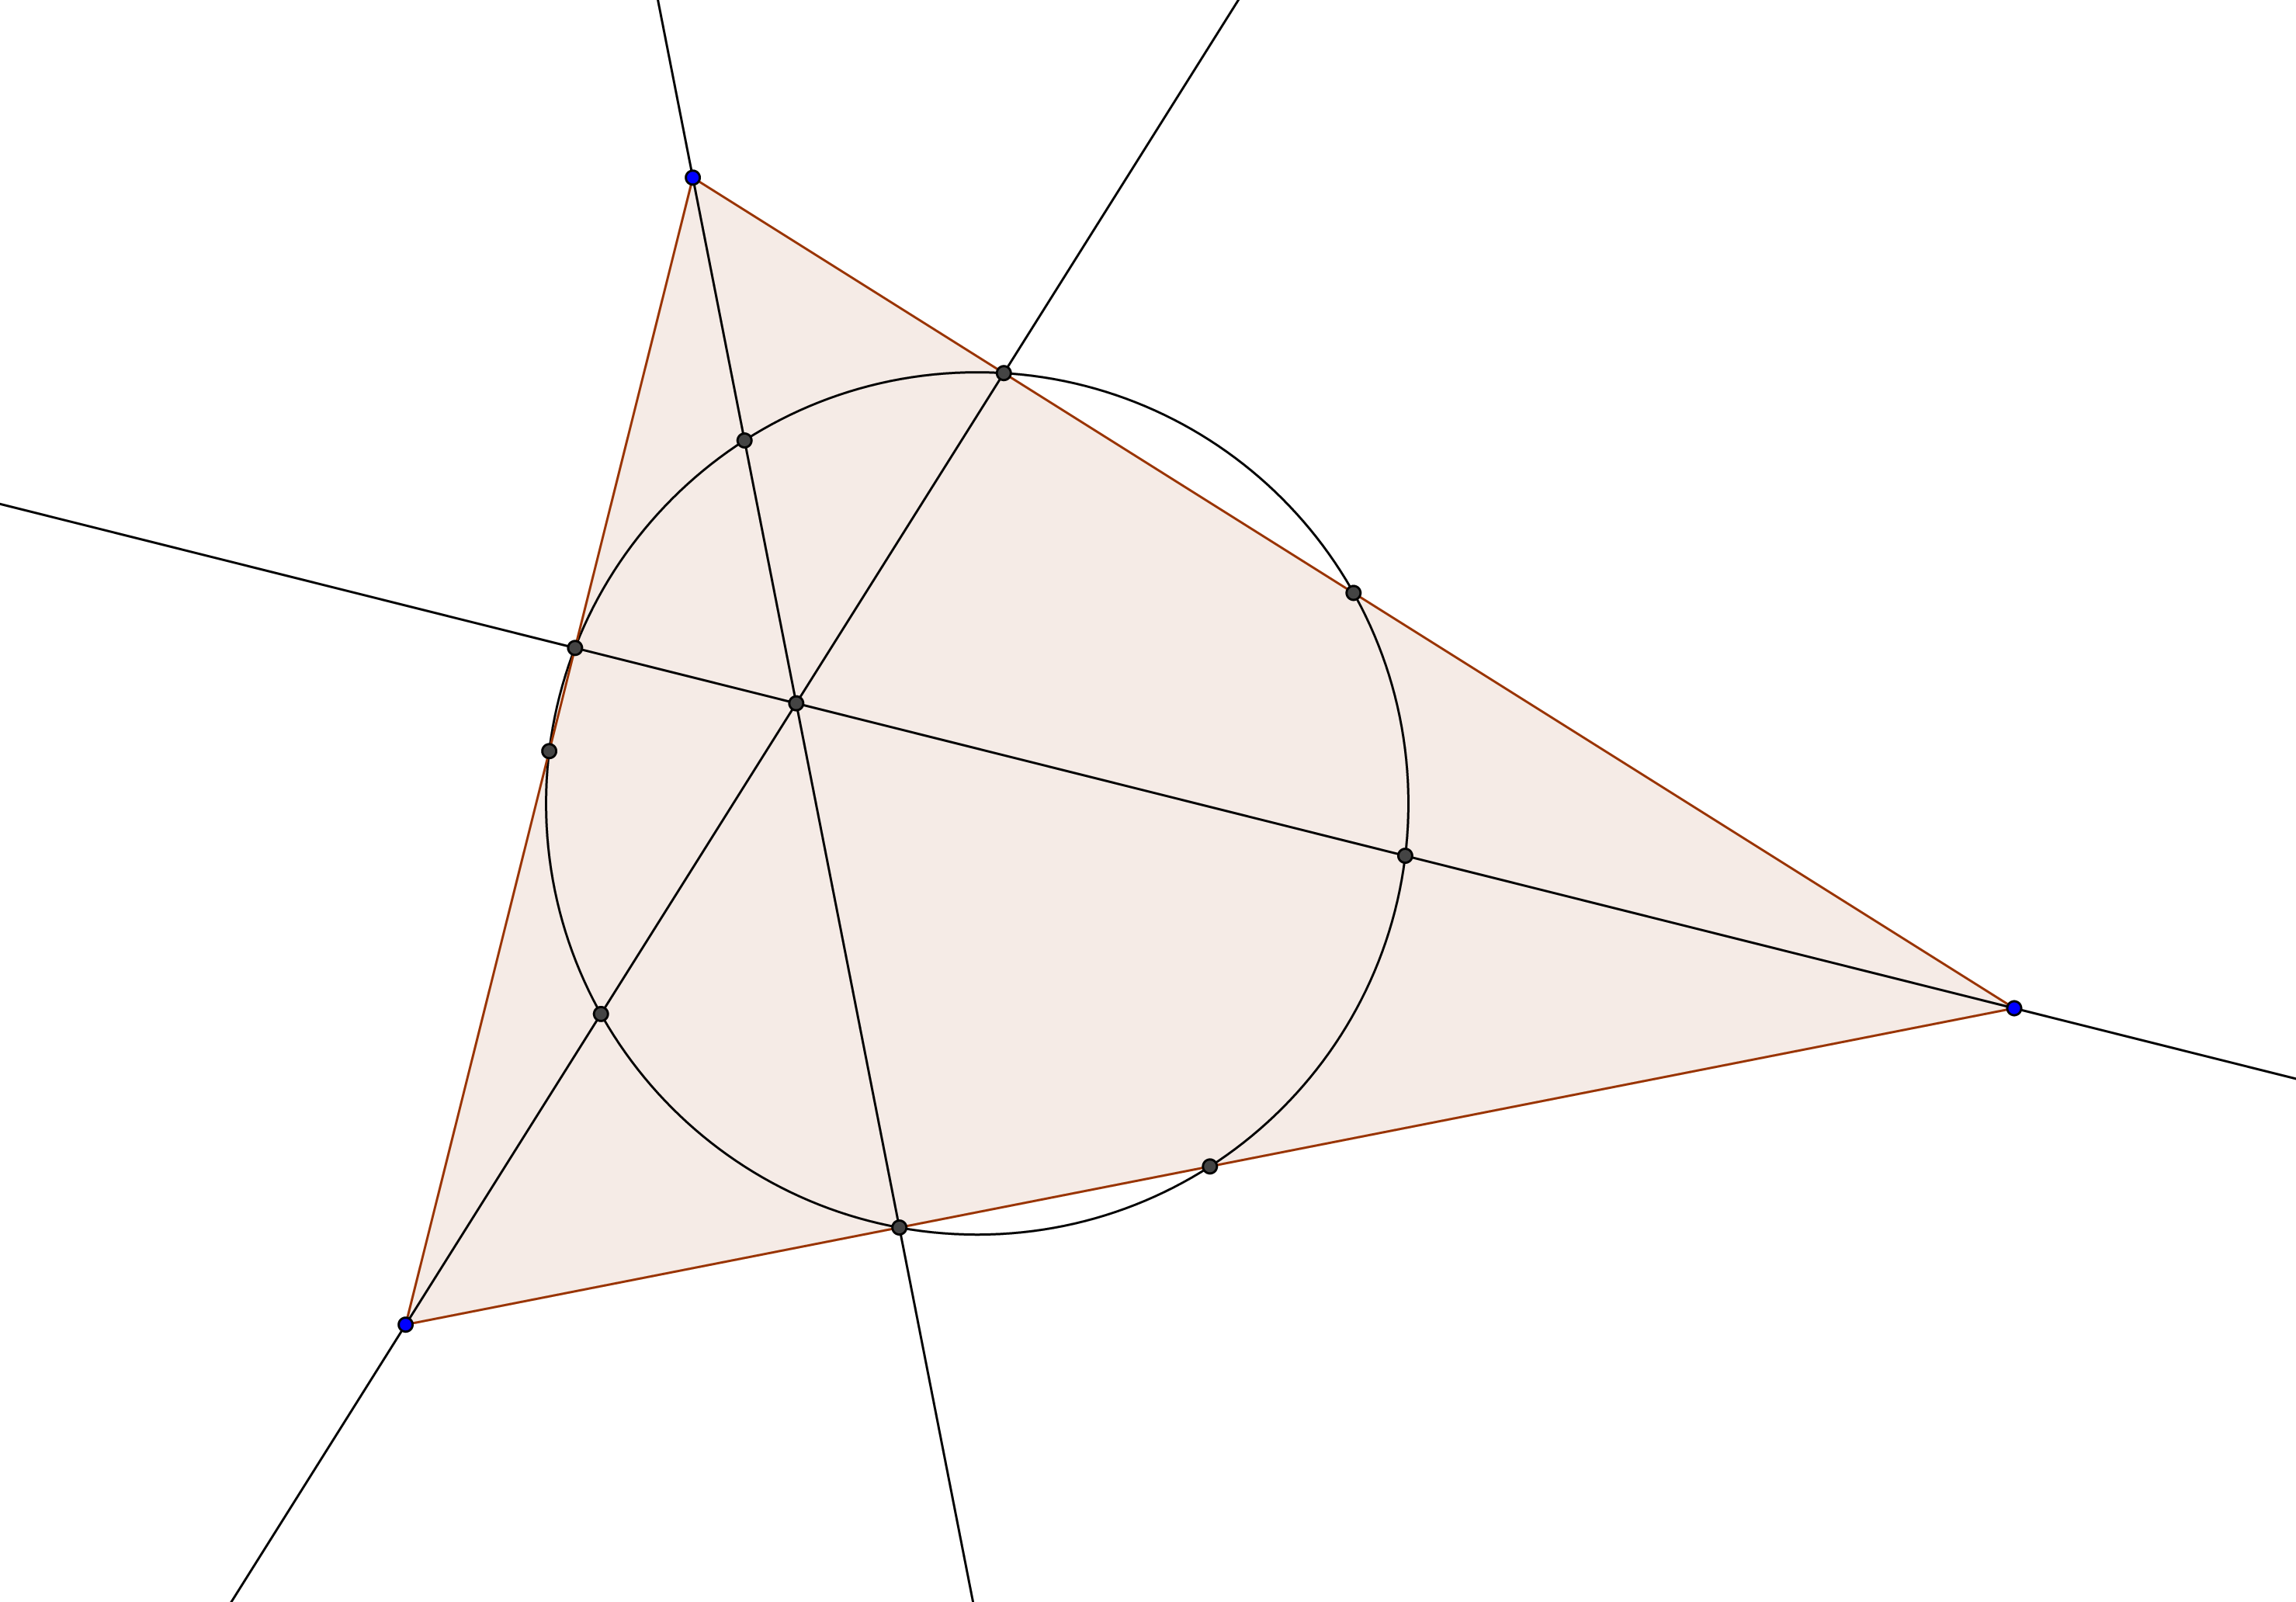
\includegraphics{NPC}
\end{marginfigure}

\setcounter{section}{6}
\renewcommand{\thesection}{\Alph{section}}
\section*{Final Examination Problems}
\thispagestyle{empty}

\marginnote{\textbf{Instructions:} 
This examination is due by noon on Thursday, December 19th. 
Be sure to adhere to the standards we have used all semester. 

You may use your course notes, the \emph{Elements} through Book IV and the class journal as references. 
You may not speak to anyone about the content of this exam except me until the deadline has passed. 
Explain yourself clearly and give complete arguments to receive full credit. You may turn in the exam by dropping it off at my office (327 Wright Hall) or at the Mathematics Department Office (220 Wright Hall).

Good Luck!}

\begin{problem} 
Given a circle and its center, construct a regular octagon inscribed in the circle. 
Prove that your construction works.
\end{problem}

\begin{definition}
A quadrilateral is called \emph{circumscriptable} if there exists a circle lying inside the quadrilateral which is tangent to each of the four sides.
\end{definition}

\begin{problem} 
Given a triangle $ABC$ and a segment $DE$, construct a rectangle with the same content as the triangle and with $DE$ as one side. 
(Do not use similarity! Use Euclidean theory of equal content.) 
Illustrate your work with well-drawn figures.
\end{problem}

\begin{problem} 
Let $ABC$ be a triangle. 
Extend sides $AB$ and $AC$ to rays $AB$ and $AC$, forming exterior angles. 
Let $r_A$ be the angle bisector of angle $BAC$, let $r_B$ be the angle bisector of the exterior angle at $B$, and let $r_C$ be the angle bisector of the exterior angle at $C$.
\begin{compactitem}
\item Prove that these three rays are concurrent.
The point just constructed is called an \emph{excenter} of $ABC$. 
Let us call it $E_A$.
\item Prove that $E_A$ is the center of a circle which is tangent to the extended sides of the triangle.
\end{compactitem}
\end{problem}

\begin{problem} Settle the following conjecture as completely as you can. I want to see as much as you can do with this.
\begin{quotation}
\textbf{Conjecture:} 
Let ABCD be a quadrilateral. 
Then $ABCD$ is circumscriptable if, and only if, $AB$ and $CD$ taken together are congruent to $AD$ and $BC$ taken together.
\end{quotation}
\end{problem}

\vfill
\end{document}
